\documentclass[aps, pre, onecolumn, a4paper, floatfix]{revtex4}
%\documentclass[twocolumn]{revtex4}
\usepackage{graphicx}
\usepackage{amsmath}
\usepackage{placeins}
\usepackage{color}
\usepackage{hyperref}
%\usepackage{bug}
%\bibliographystyle{plain}




\begin{document}

\title{Supplemental materials}
\author{Sebastian M. Krause}
\author{Vinko Zlati\'{c}}
\affiliation{Theoretical Physics Division, Rudjer Bo\v{s}kovi\'{c} Institute, Zagreb, Croatia}
\author{Michael M. Danziger}
\affiliation{Department of Physics, Bar Ilan University, Ramat Gan, Israel}
\begin{abstract}

\end{abstract}
%\pacs{89.65.-s, 05.50.+q, 05.65.+b, 64.60.De}
\maketitle

\section*{List of variables}
{\centering

\begin{tabular}{ c c }
 \hline
 \multicolumn{2}{ c } {Networks}\\
 \hline
 $N$ & Number of nodes \\
 $\bar k$ & Average degree \\
 $k_i$ & Degree of node $i$ \\
 $p_k$ & Degree distribution \\
 $\alpha$ & Exponent of scale free degree distribution \\
 $g_0$ & Generating function of degree \\
 $g_1$ & Generating function of excess degree \\
 \hline
 \multicolumn{2}{ c } {Colors}\\
 \hline
 $C$ & Number of colors \\
 $c\in 1,2,\dots C$ & A color \\
 $r_c$ & Color distribution \\
 $n_{\rm deg}$ & Degeneration of the highest color frequency \\
 ${\tilde r}_{c,k}$ & degree-dependent color distribution \\
 \hline
 \multicolumn{2}{ c } {Standard percolation ingredients}\\
 \hline
 ${\mathcal G}$ & Set of nodes in the giant component (color blind) \\
 $u$ & Prob.\ of not being connected to giant comp.\ over a link \\
 $S$ & Size of giant component \\
 $\phi_{\bar c}$ & Fraction of nodes without color $c$ \\
 ${\mathcal G}_{\bar c}$ & Set of nodes in the giant component avoiding color c \\
 $u_{\bar c}$ & Prob.\ of not being connected to color avoiding giant comp.\ over a link \\
 $S_{\bar c}$ & Size of color avoiding giant component \\
 \hline
 \multicolumn{2}{ c } {Percolation over color avoiding paths}\\
 \hline
 ${\mathcal G}_{\rm color}$ & Set of nodes which can communicate avoiding all colors \\
 $S_{\rm color}$ & Size of this component \\
 $B_{k,k'}$ & Prob.\ that out of $k$ links $k'$ connect to giant component \\
 $M_{k',\vec \kappa}$ & Prob.\ that out of $k'$ links $\kappa_1$ connect to color 1 etc. \\
 $P_{\vec \kappa}$ & Success probability having neighbors of colors acc. to $\vec \kappa$ \\
 $U_{\bar c}$ & Prob.\ that a link fails connecting to ${\mathcal G}_{\rm color}$ which already connects to ${\mathcal G}$ \\
 $S_{{\rm color},\infty}$ & Size of the set of all nodes being connected to giant component over two links or more \\
 \hline
 \hline
 $\beta$ & Critical exponent \\
 ${\bar k}_{\rm crit}$ & Critical value of average degree \\
 $k_{\rm step}$ & Degree above which all nodes have the same color \\
 $\gamma$ & Fraction of nodes with highest degree \\
\end{tabular}

}





\section{Size of giant avoidable colors component in the configuration model}

\subsection{Graph ensembles with color distributions}

\subsection{Question and connection to percolation theory}

\begin{figure}[htb]
  \begin{minipage}[b]{0.18\linewidth}
    \begin{center}
      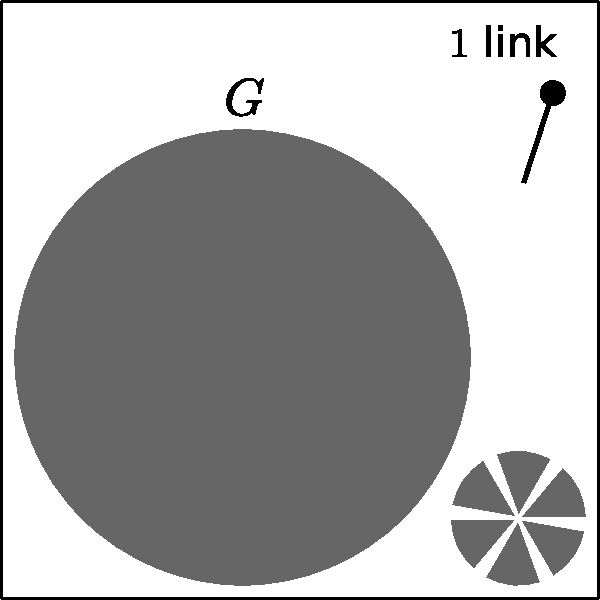
\includegraphics[width=0.99\columnwidth]{sets_gc_all1.pdf}
   \end{center}
  \end{minipage}
  \begin{minipage}[b]{0.05\linewidth}
    \begin{center}
      {\Large $\xrightarrow{u}$}\\
      \vspace{15mm}
    \end{center}
  \end{minipage}
  \begin{minipage}[b]{0.18\linewidth}
    \begin{center}
      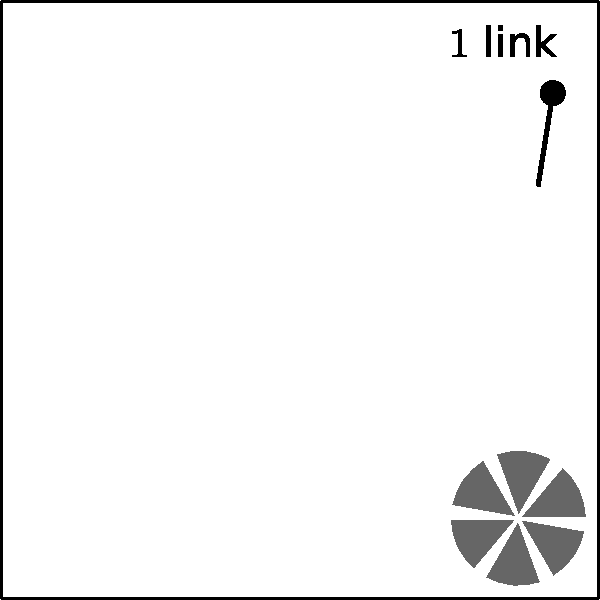
\includegraphics[width=0.99\columnwidth]{sets_gc_no1.pdf}
    \end{center}
  \end{minipage}
  \begin{minipage}[b]{0.05\linewidth}
  \ 
  \end{minipage}
  \begin{minipage}[b]{0.18\linewidth}
    \begin{center}
      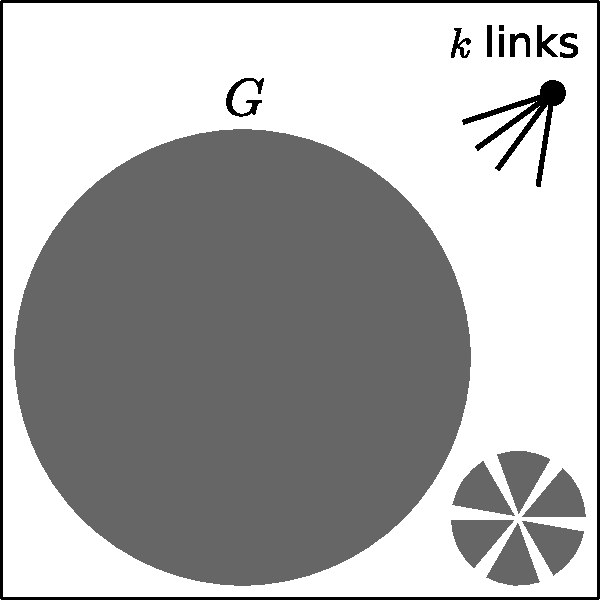
\includegraphics[width=0.99\columnwidth]{sets_gc_allk.pdf}
    \end{center}
  \end{minipage}
  \begin{minipage}[b]{0.07\linewidth}
    \begin{center}
      {\Large $\xrightarrow{1-u^k}$}\\
      \vspace{15mm}
    \end{center}
  \end{minipage}
  \begin{minipage}[b]{0.18\linewidth}
    \begin{center}
      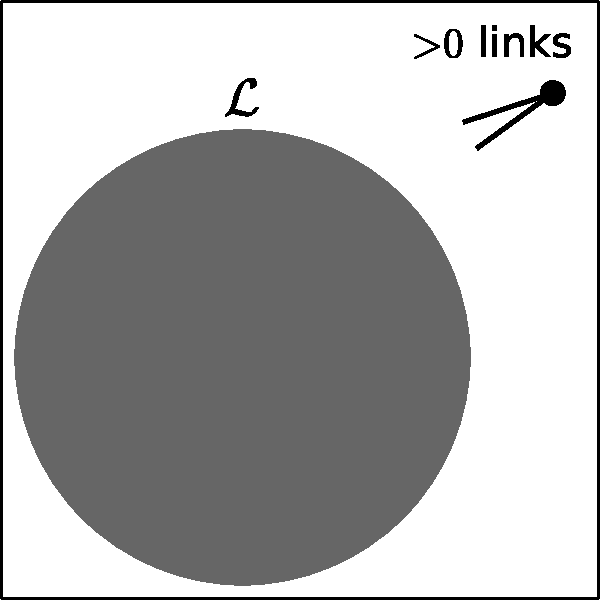
\includegraphics[width=0.99\columnwidth]{sets_gc_gck.pdf}
    \end{center}
  \end{minipage}
    \caption{We base our theory on the method to calculate the size of 
    normal giant components, as illustrated in this figure. Using a self 
    consistency equation, the probability $u$ can be calculated. This is the 
    probability, that a node is not connected to the giant component over a 
    single link (see on the left). On the right, the probability for a node 
    with $k$ links is illustrated to have at least one link connecting to 
    the giant component. $u^k$ is the probability that all links fail.}
    \label{fig:1}
\end{figure}




\begin{figure}[htb]
  \begin{minipage}[b]{0.245\linewidth}
    \begin{center}
    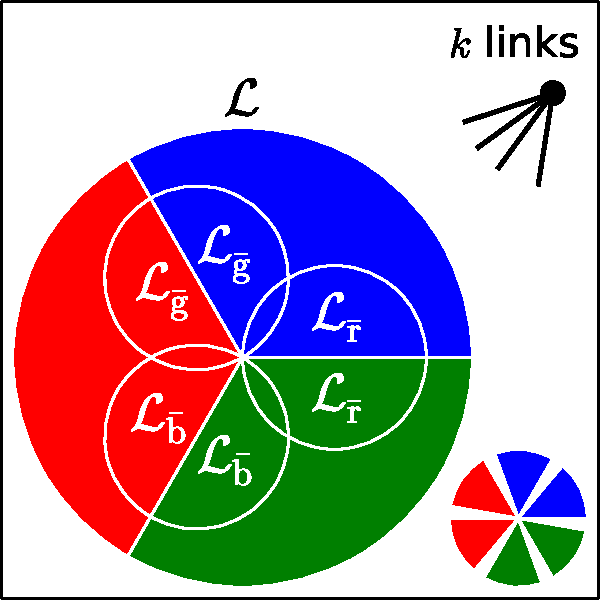
\includegraphics[width=0.99\columnwidth]{sets_k_all.pdf}
   \end{center}
  \end{minipage}
  \begin{minipage}[b]{0.1\linewidth}
    \begin{center}
      {\Large $\xrightarrow{?}$}\\
      \vspace{20mm}
    \end{center}
  \end{minipage}
  \begin{minipage}[b]{0.6\linewidth}
    \begin{center}
    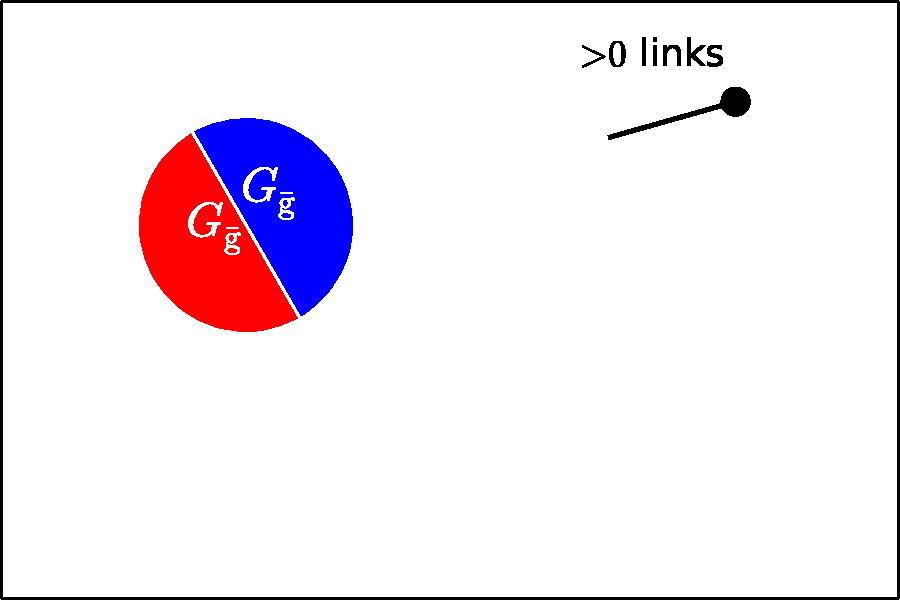
\includegraphics[height=0.4\columnwidth]{sets_k_gc_no_2.pdf}
     \hspace{-1mm}
    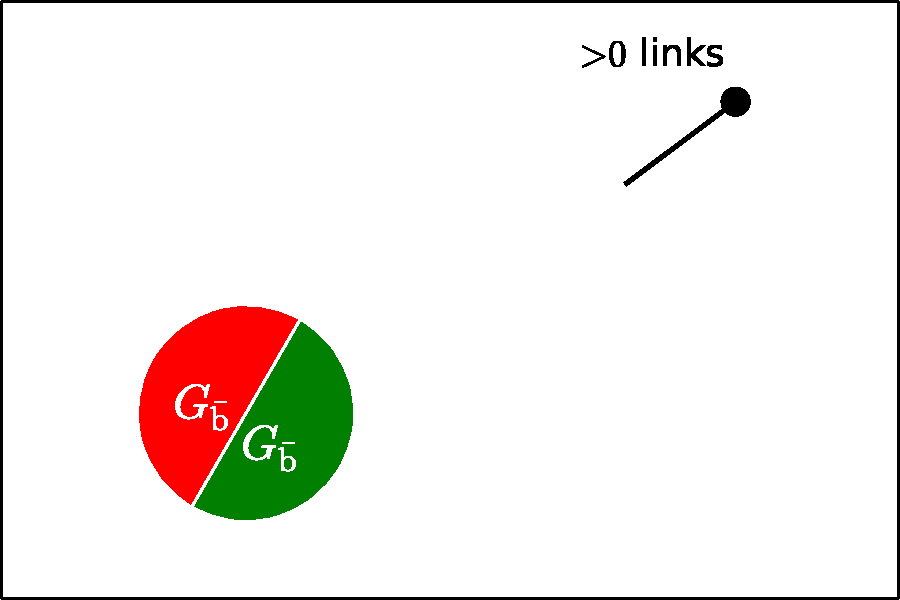
\includegraphics[trim=100 0 0 0,clip,height=0.4\columnwidth]{sets_k_gc_no_3.pdf}
     \hspace{-1mm}
    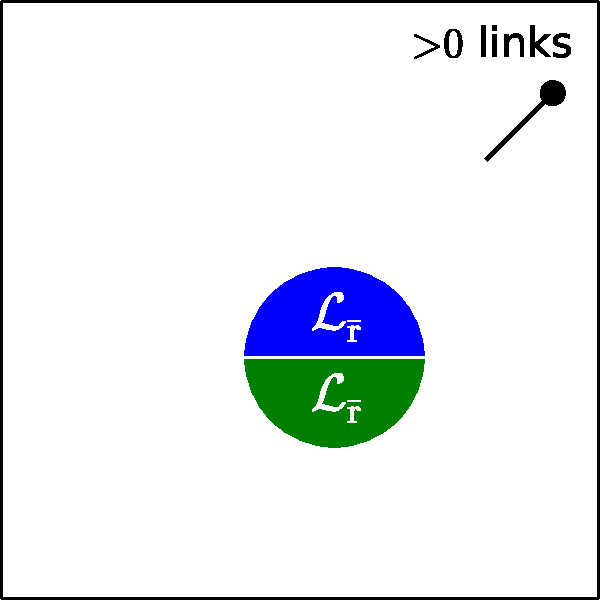
\includegraphics[trim=100 0 0 0,clip,height=0.4\columnwidth]{sets_k_gc_no_1.pdf}
   \end{center}
  \end{minipage}
    \caption{We have to calculate the probability, if a node with $k$ links is 
    for every color $c$ connected to the giant component $G_{\bar c}$ with deleted 
    color $c$. All connections over at least one link have to exist at the same 
    time. We illustrate this question with the three colors red ($c=$r), green 
    ($c=$g) and blue ($c=$b). If a link connects to $G_{\bar{\rm g}}$, it for 
    sure does not connect to $G_{\bar c}$ for one of the other colors. This kind of 
    dependence forces us to use a stepwise calculation with conditional probabilities.}
    \label{fig:1}
\end{figure}


%
For estimating the size of the largest avoidable colors component analytically, results from percolation 
theory can be used. First of all, the existence of a (colorblind) giant component clearly is a 
prerequisite for the existence of a macroscopic fraction of successful node pairs. With the 
generating functions of degree $g_0(z)=\sum_k p_k z^k$ and excess degree 
$g_1(z)=\sum_k q_k z^k$, the size of the giant component $S$ can be calculated (assuming infinite
networks which are locally treelike) using 
the average probability $u$, ``that a vertex is not connected to the giant component 
via its connection to some particular neighboring vertex'' (Newman, page 461): 
\begin{align}
u &= g_1(u)\\
S &= 1 - g_0(u).\label{eq:gc}
\end{align}
Lets call the set of all nodes belonging to the giant component as ${\mathcal G}$. 

As we have tested numerically that $S_{\rm color}$ can be used to describe the success of node 
pairs in connecting over paths with avoided colors, it is useful to assess this quantity 
analytically. We will do this assuming an infinite, locally treelike network. 
We calculate $S_{\rm color}$ as the probability, that a randomly chosen node belongs to 
${\mathcal G}_{\rm color}$. 

Let us start with the standard percolation theory. We can rewrite eq.~\ref{eq:gc} for the size of 
the giant component as 
%%%
\begin{align}
S &= \sum_{k=0}^{\infty}p_k \sum_{k'=0}^{k} B_{k,k'} \times \left( 1-\delta_{k',0}\right),\\
B_{k,k'} &={k \choose k'}(1-u)^{k'}u^{k-k'},
\end{align}
%%%
where $p_k$ is the probability that a randomly chosen node has exactly $k$ links and $B_{k,k'}$
is the binomial probability that out of these links $k'$ links connect to the giant component. The 
success probability $\left( 1-\delta_{k',0}\right)$ is zero 
if there is no link connecting to the giant component and one else. 


\subsection{One link probabilities}



\begin{figure}[htb]
   \begin{center}
    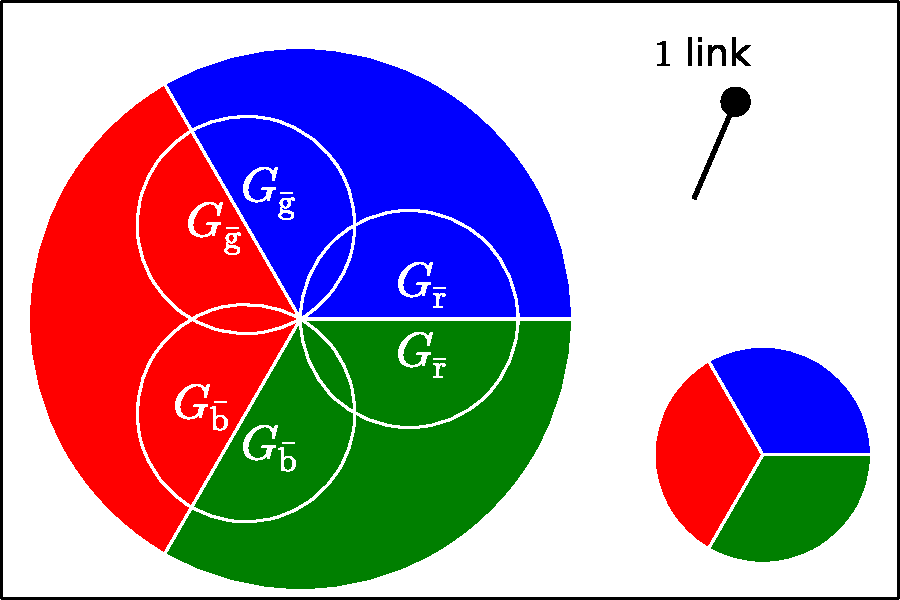
\includegraphics[width=0.22\columnwidth]{sets_1_all.pdf}
    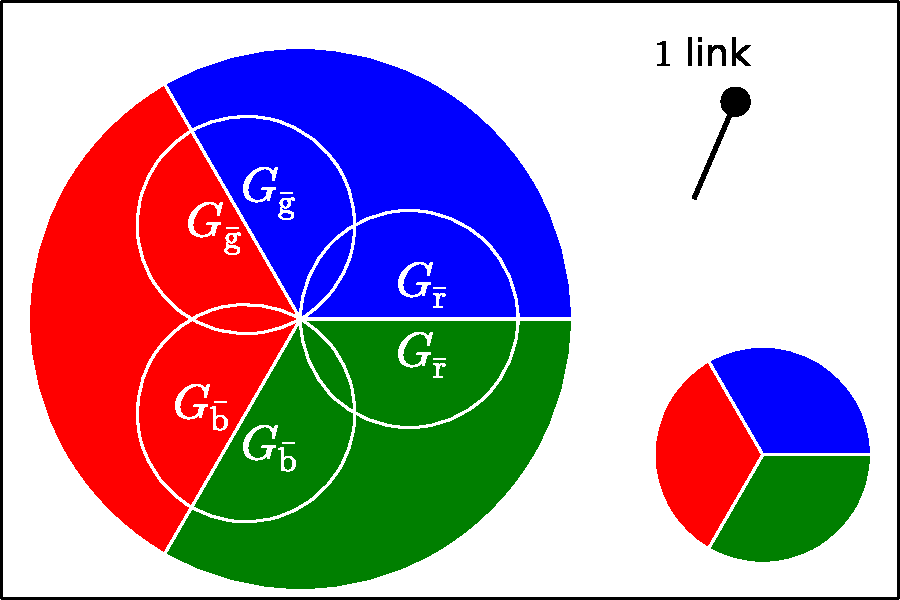
\includegraphics[width=0.22\columnwidth]{sets_1_all.pdf}
    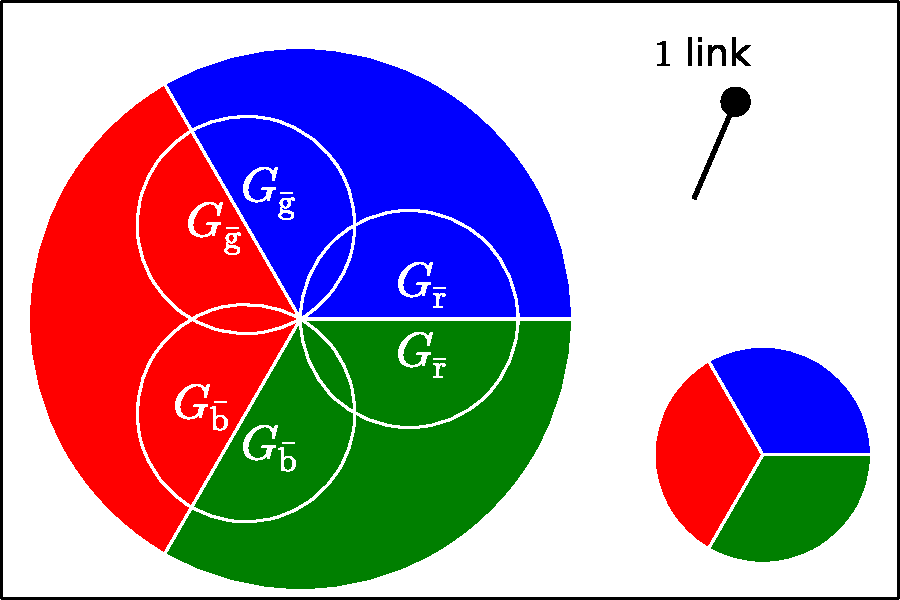
\includegraphics[width=0.22\columnwidth]{sets_1_all.pdf}
    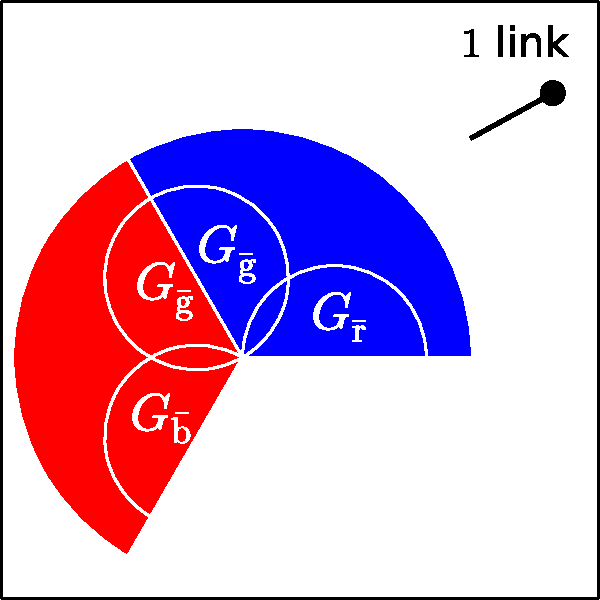
\includegraphics[width=0.22\columnwidth]{sets_1_no_2_gc.pdf}\\
     \vspace{3mm}
      {\large \hspace{5mm} $\downarrow u$\hspace{34mm}$\downarrow r_{\rm g}$ 
      \hspace{34mm}$\downarrow u_{\bar{\rm g}}$ \hspace{34mm}$\downarrow U_{\bar{\rm g}}$}\\
     \vspace{3mm}
    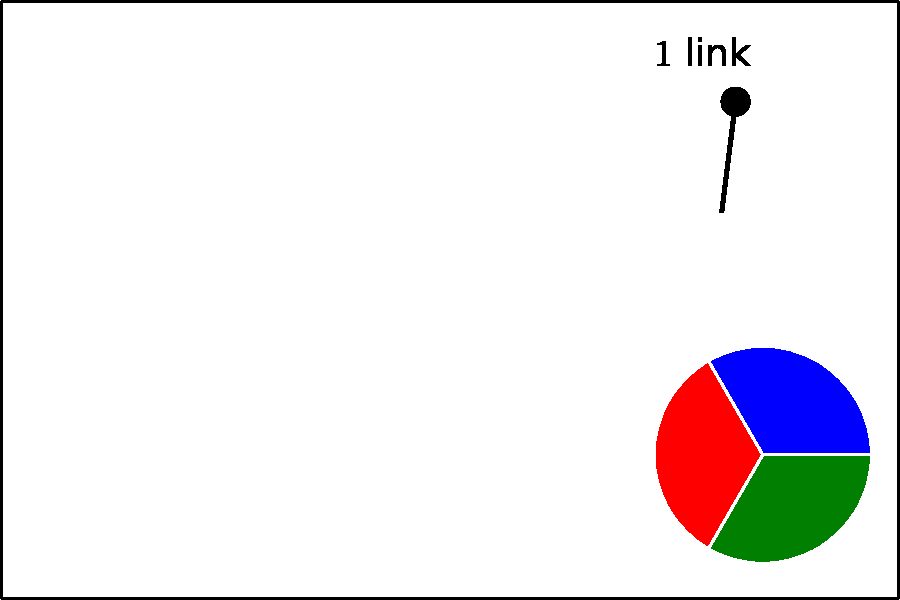
\includegraphics[width=0.22\columnwidth]{sets_1_no_gc.pdf}
    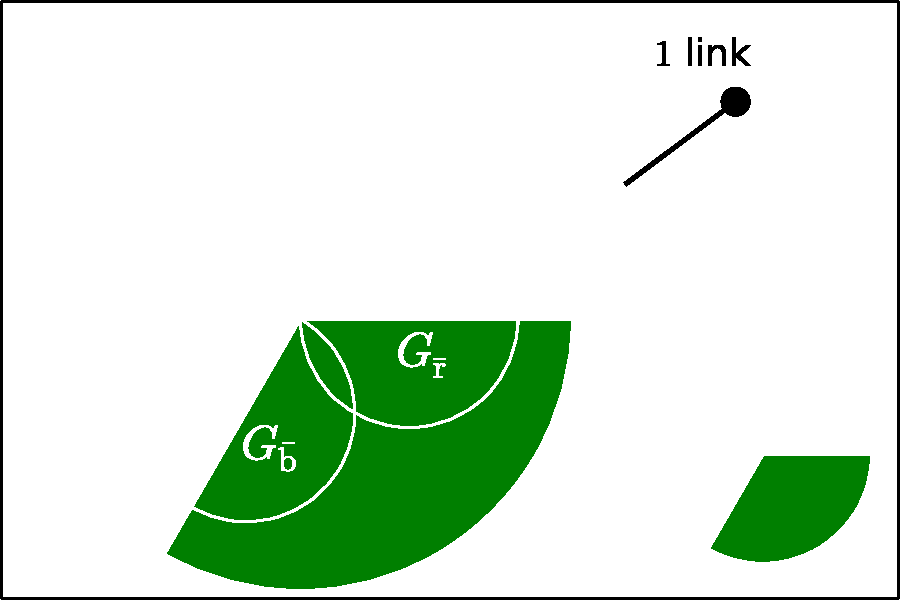
\includegraphics[width=0.22\columnwidth]{sets_1_c2.pdf}
    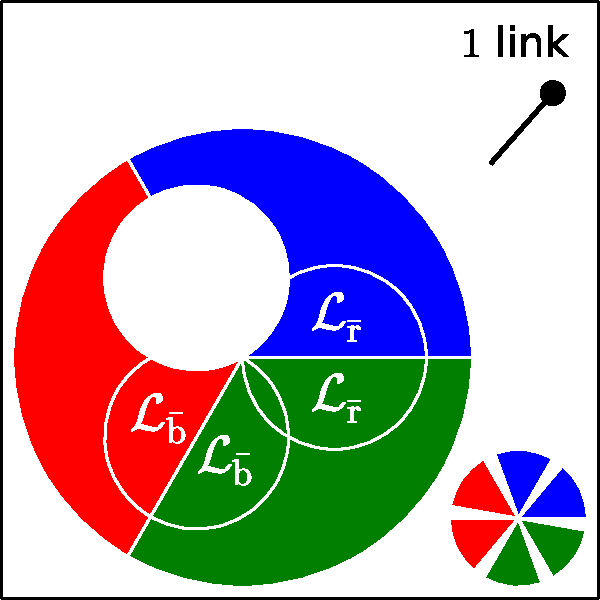
\includegraphics[width=0.22\columnwidth]{sets_1_gc_no_gc_no_2.pdf}
    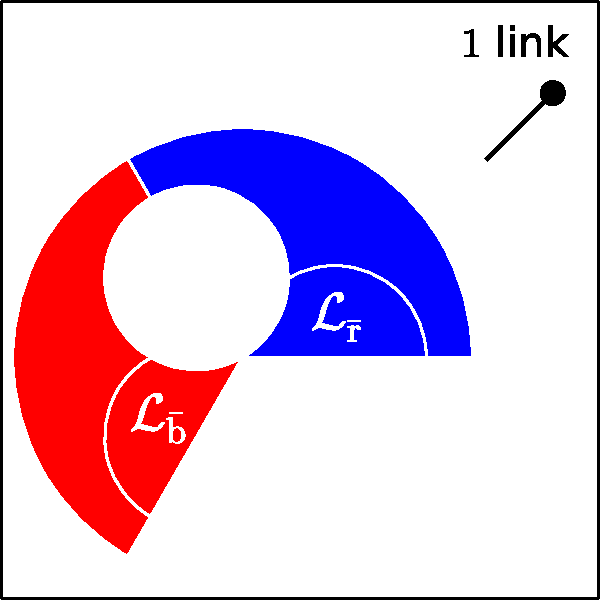
\includegraphics[width=0.22\columnwidth]{sets_1_no_2_gc_no.pdf}
   \end{center}
  \caption{Probabilities for a single link to connect to different parts of the network. We 
  use these probabilities as primitives to calculate the probability for many links. While 
  $u$, $r_c$ and $u_{\bar c}$ can be calculated with standard methods invented for the 
  configuration model before, the conditional probability $U_{\bar c}$ can be calculated as 
  a combination of the others.}
  \label{fig:primitives}
\end{figure}

Another prerequisite is the existence of a giant component after deleting all nodes of one 
of the colors $c$. Lets call the analogue of $u$ after all nodes of color $c$ are 
deleted as $u_{\bar c}$, the set of all nodes in the remaining giant component as 
${\mathcal G}_{\bar c}$, and its size as $S_{\bar c}$. 
We have 
\begin{align}
\phi_{\bar c} &= 1-r_c\\
u_{\bar c} &= 1-\phi_{\bar c} + \phi_{\bar c} g_1(u_{\bar c})\label{eq:u_c}\\
S_{\bar c} &= \phi_{\bar c} (1-g_0(u_{\bar c})).
\end{align}
Finally a node pair is for sure successful, if for both nodes the following 
holds: For every color $c$ there exists at least one neighbor belonging to 
${\mathcal G}_{\bar c}$. The set of all nodes fulfilling this 
condition is $L_{\rm color}$, and its size as $S_{\rm color}$. 

According to the choices we have made so far, those links connect to the giant component 
${\mathcal G}$ and none of the nodes they are connecting to has color $c$. Therefore, a single 
of those links fails in connecting to ${\mathcal G}_{\bar c}$ with the conditional probability 
%%%
\begin{align}
U_{\bar c} &= 1 - \frac{1-u_{\bar c}}{(1-u)(1-r_c)}.\label{eq:U_c}
\end{align}
%%%
The last term is the probability, that over a single link a connection to ${\mathcal G}_{\bar c}$
is established, if this link already fulfills the following precondition: 
It connects to ${\mathcal G}$ and at the same time to a node without color $c$. 
This precondition has probability $(1-u)(1-r_c)$, as colors are randomly distributed and therefore 
are not correlated with the probability $u$ or $1-u$. As the links connecting to ${\mathcal G}_{\bar c}$ 
are a subset of all links fulfilling the precondition, the conditional probability can be 
calculated by dividing with the probability of the precondition. 
Notice that the additional information of the explicit color, instead of only stating that the color 
is not $c$, does not alter the results, as a further restriction of the colors 
would meat the numerator and denominator identically and therefore would cancel out. 


\begin{figure}[htb]
  \begin{minipage}[b]{0.22\linewidth}
    \begin{center}
    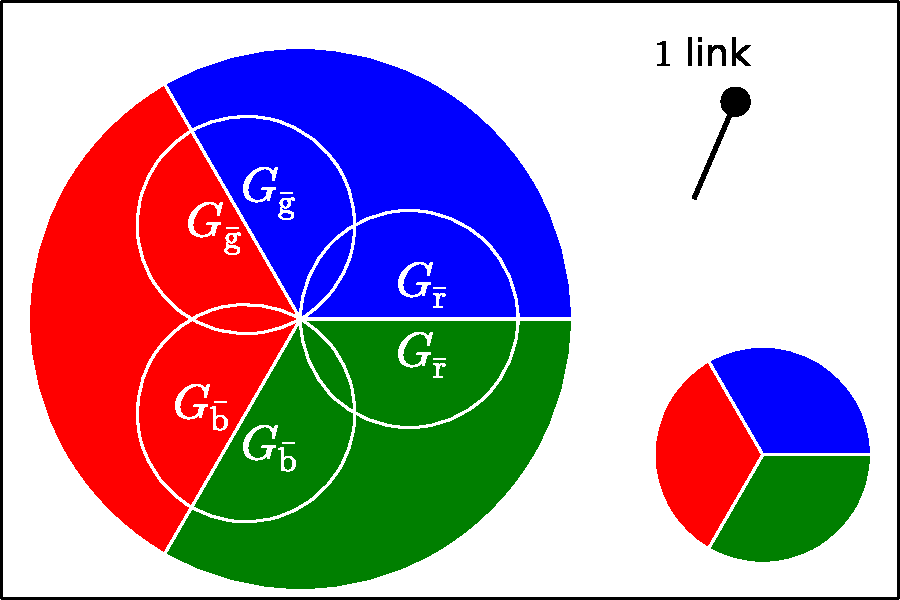
\includegraphics[width=0.99\columnwidth]{sets_1_all.pdf}\\
      \vspace{50mm}
   \end{center}
  \end{minipage}
  \begin{minipage}[b]{0.15\linewidth}
    \begin{center}
      $(1-u)(1-r_{\rm g})$\\
      {\Large $\rightarrow$\\}
      \vspace{20mm}
      $1-u_{\bar{\rm g}}$\\
      {\Large $\searrow$\\}
      \vspace{35mm}
    \end{center}
  \end{minipage}
  \begin{minipage}[b]{0.22\linewidth}
    \begin{center}
    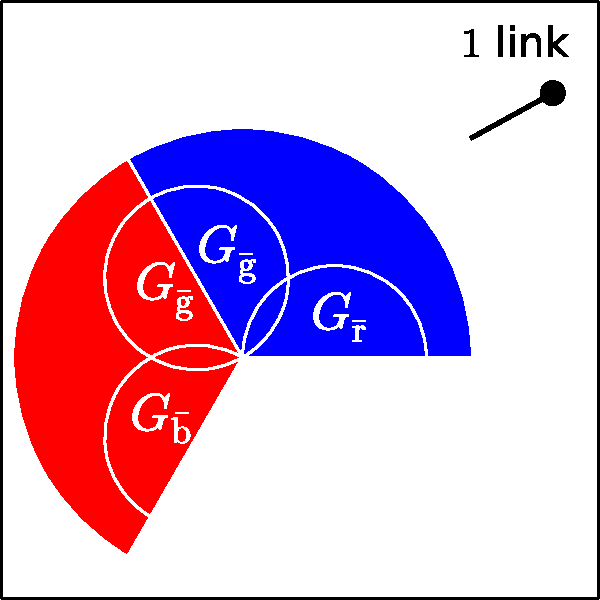
\includegraphics[width=0.99\columnwidth]{sets_1_no_2_gc.pdf}\\
     \vspace{3mm}
    {\large $\downarrow$} $1-U_{\bar{\rm g}}$\\
     \vspace{3mm}
    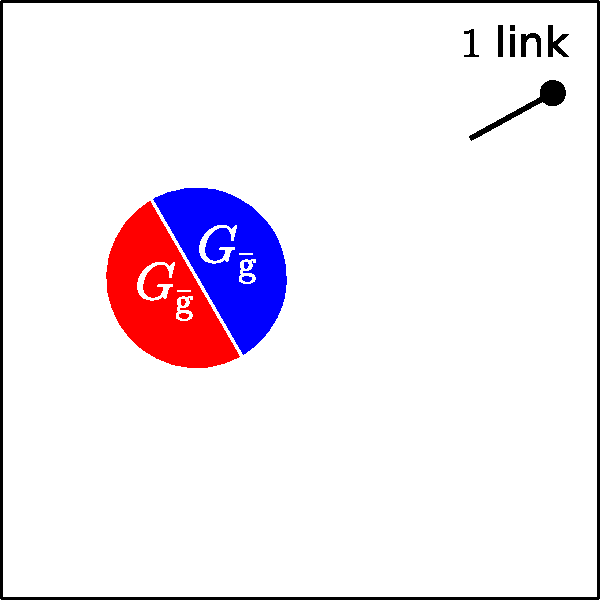
\includegraphics[width=0.99\columnwidth]{sets_1_gc_no_2.pdf}\\
   \end{center}
  \end{minipage}
    \caption{This figure illustrates the calculation of $U_{\bar{\rm g}}$ 
    using the equality $(1-u)(1-r_{\rm g})(1-U_{\bar{\rm g}})=1-u_{\bar{\rm g}}$. For 
    that, we have assumed independence of the qualities of the link under 
    consideration, especially of the color it connects to and if it connects to 
    the giant component. }
    \label{fig:1}
\end{figure}



\subsection{Averaging over link distributions}




\begin{figure}[htb]
  \begin{minipage}[b]{0.245\linewidth}
    \begin{center}
    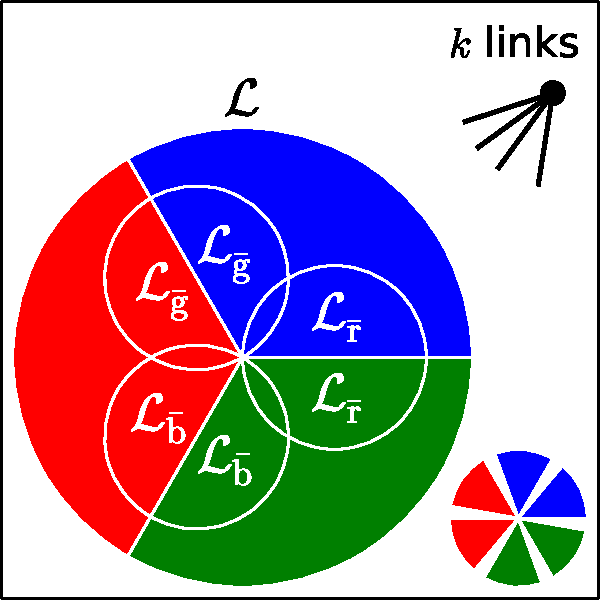
\includegraphics[width=0.99\columnwidth]{sets_k_all.pdf}
   \end{center}
  \end{minipage}
  \begin{minipage}[b]{0.1\linewidth}
    \ 
  \end{minipage}
  \begin{minipage}[b]{0.6\linewidth}
    \begin{center}
    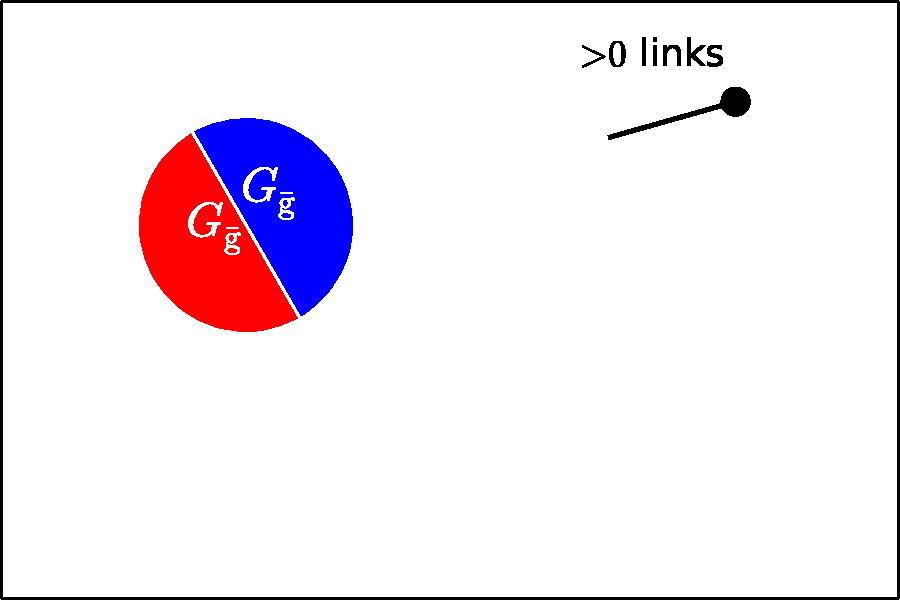
\includegraphics[height=0.4\columnwidth]{sets_k_gc_no_2.pdf}
     \hspace{-1mm}
    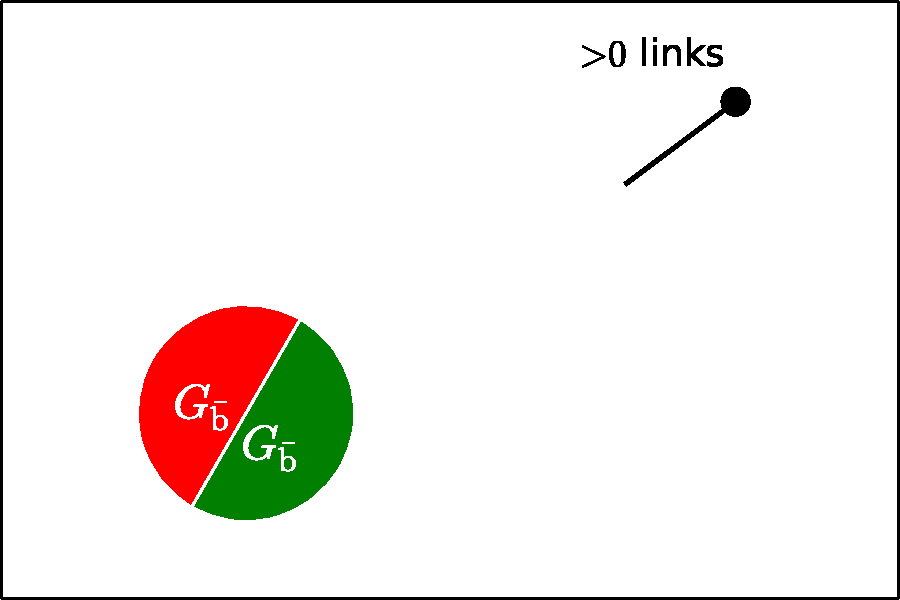
\includegraphics[trim=100 0 0 0,clip,height=0.4\columnwidth]{sets_k_gc_no_3.pdf}
     \hspace{-1mm}
    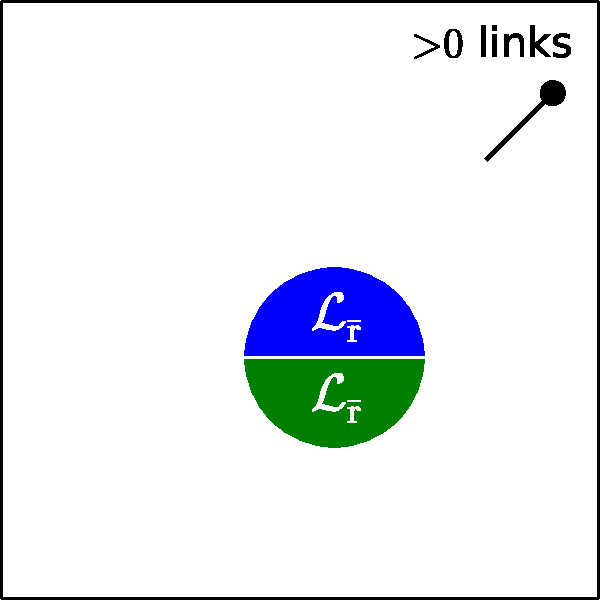
\includegraphics[trim=100 0 0 0,clip,height=0.4\columnwidth]{sets_k_gc_no_1.pdf}
   \end{center}
  \end{minipage}\\
     \vspace{3mm}
      {\large \hspace{-30mm} $\downarrow B_{k,k'}$\hspace{90mm}$\uparrow P_{\vec \kappa}$ }\\
     \vspace{3mm}
  \begin{minipage}[b]{0.245\linewidth}
    \begin{center}
    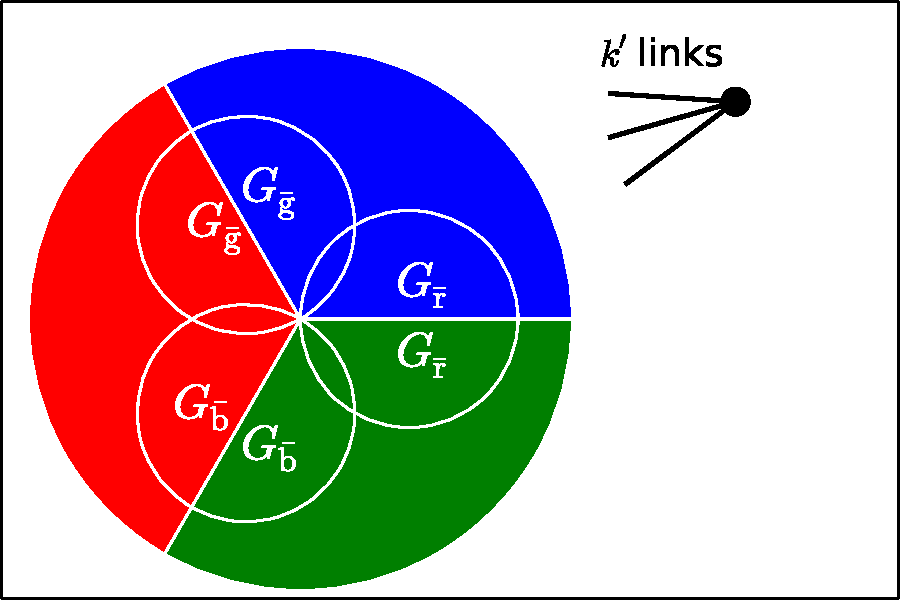
\includegraphics[width=0.99\columnwidth]{sets_k_gc.pdf}
   \end{center}
  \end{minipage}
  \begin{minipage}[b]{0.1\linewidth}
    \begin{center}
      {\Large $\xrightarrow{M_{k',\vec{\kappa}}}$}\\
      \vspace{20mm}
    \end{center}
  \end{minipage}
  \begin{minipage}[b]{0.6\linewidth}
    \begin{center}
    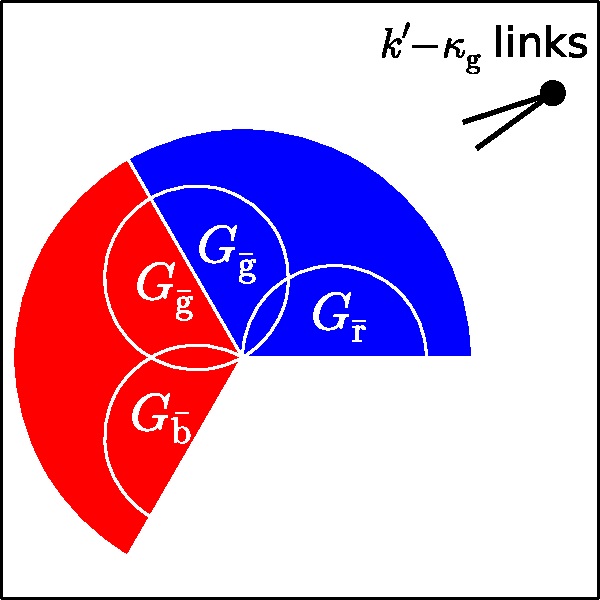
\includegraphics[height=0.4\columnwidth]{sets_k_no_2_gc.pdf}
     \hspace{-1mm}
    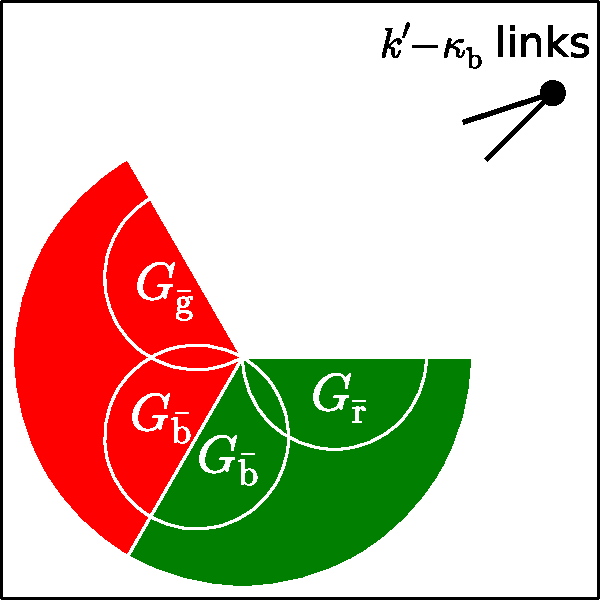
\includegraphics[trim=100 0 0 0,clip,height=0.4\columnwidth]{sets_k_no_3_gc.pdf}
     \hspace{-1mm}
    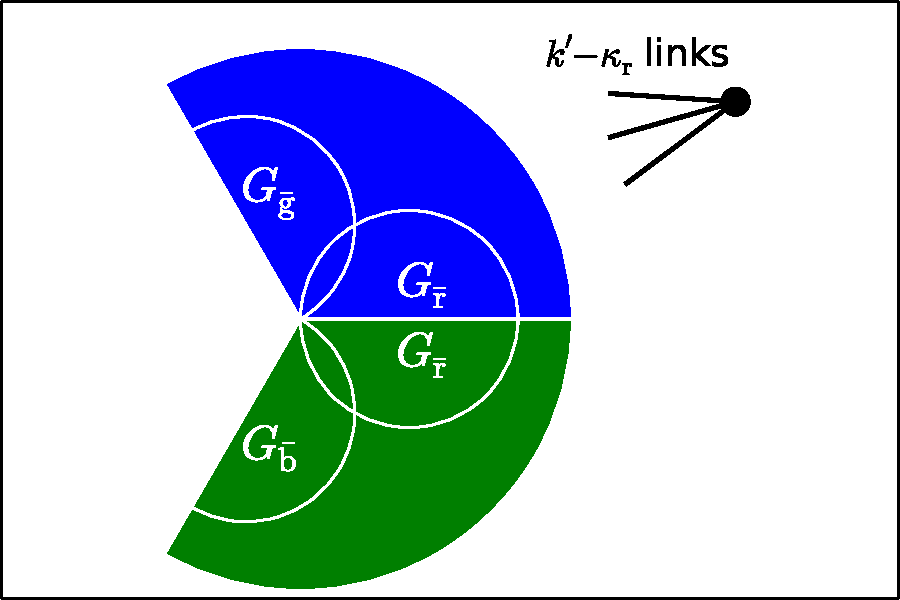
\includegraphics[trim=100 0 0 0,clip,height=0.4\columnwidth]{sets_k_no_1_gc.pdf}
   \end{center}
  \end{minipage}
    \caption{For calculating the probability of a node with $k$ links to belong to 
    $G_{\rm color}$, we have to average over different link constellations which this node 
    might show. First, $B_{k,k'}$ is the probability that out of the $k$ links $k'$ 
    connect to the giant component. It is calculated using $u$ (compare figure~\ref{fig:primitives} 
    on the left). Second, $M_{k',\vec{\kappa}}$ gives the probability for a certain color 
    distribution among the links. It is calculated using $r_{\rm g}$ etc. (compare 
    figure~\ref{fig:primitives}, second from left). We assume that this second step is 
    independent of the first step, what is confirmed with the final results. Third, 
    $P_{\vec \kappa}$ gives the joint probability that for this color distribution 
    $G_{\bar{\rm r}}$, $G_{\bar{\rm b}}$ and $G_{\bar{\rm g}}$ are connected to at 
    the same time. This is calculated using $U_{\bar{\rm r}}$ etc. (compare 
    figure~\ref{fig:primitives} on the right). We tested numerically that e.g. 
    $U_{\bar{\rm r}}$ and $U_{\bar{\rm b}}$ are independent for a link connecting 
    to the giant component and color green.}
    \label{fig:1}
\end{figure}




As we have tested numerically that $S_{\rm color}$ can be used to describe the success of node 
pairs in connecting over paths with avoided colors, it is useful to assess this quantity 
analytically. We will do this assuming an infinite, locally treelike network. 
We calculate $S_{\rm color}$ as the probability, that a randomly chosen node belongs to 
${\mathcal G}_{\rm color}$. 

Let us start with the standard percolation theory. We can rewrite eq.~\ref{eq:gc} for the size of 
the giant component as 
%%%
\begin{align}
S &= \sum_{k=0}^{\infty}p_k \sum_{k'=0}^{k} B_{k,k'} \times \left( 1-\delta_{k',0}\right),\\
B_{k,k'} &={k \choose k'}(1-u)^{k'}u^{k-k'},
\end{align}
%%%
where $p_k$ is the probability that a randomly chosen node has exactly $k$ links and $B_{k,k'}$
is the binomial probability that out of these links $k'$ links connect to the giant component. The 
success probability $\left( 1-\delta_{k',0}\right)$ is zero 
if there is no link connecting to the giant component and one else. 
For our problem, this last term has to be replaced. In order to calculate 
the probability that the $k'$ links connect to all components ${\mathcal G}_{\bar c}$, 
we first have to consider the distribution of colors among the nodes these links connect to. 
%%%
\begin{align}
M_{k',\vec \kappa} &=\frac{k'!}{\kappa_1! \times \dots \times \kappa_C!} \,
(r_1)^{\kappa_1} \times \dots \times (r_C)^{\kappa_C}\,
\delta_{k',\kappa_1+\dots + \kappa_C}\label{eq:R_kk}
\end{align}
%%%
denotes the multivariate probability that out of those $k'$ links $\kappa_1$ connect to nodes of 
color 1, $\kappa_2$ links connect to nodes of color 2 etc. We define $P_{\vec \kappa}$ as the 
success probability to connect to all components ${\mathcal G}_{\bar c}$ given $\vec \kappa$. 
With this quantity, which will be evaluated below, we finally can write 
%%%
\begin{align}
S_{\rm color} &= \sum_{k=0}^{\infty}p_k \sum_{k'=0}^{k} B_{k,k'} 
\sum_{\kappa_1,\dots, \kappa_C=0}^{k'} M_{k',\vec \kappa} 
P_{\vec \kappa}.\label{eq:s_color}
\end{align}

For evaluating $P_{\vec \kappa}$, lets first concentrate on one color $c$. We have 
$\sum_{c'\neq c}\kappa_{c'}$ links which potentially can connect to the desired component ${\mathcal G}_{\bar c}$. 
According to the choices we have made so far, those links connect to the giant component 
${\mathcal G}$ and none of the nodes they are connecting to has color $c$. Therefore, a single 
of those links fails in connecting to ${\mathcal G}_{\bar c}$ with the conditional probability 
%%%
\begin{align}
U_{\bar c} &= 1 - \frac{1-u_{\bar c}}{(1-u)(1-r_c)}.\label{eq:U_c}
\end{align}
%%%
The last term is the probability, that over a single link a connection to ${\mathcal G}_{\bar c}$
is established, if this link already fulfills the following precondition: 
It connects to ${\mathcal G}$ and at the same time to a node without color $c$. 
This precondition has probability $(1-u)(1-r_c)$, as colors are randomly distributed and therefore 
are not correlated with the probability $u$ or $1-u$. As the links connecting to ${\mathcal G}_{\bar c}$ 
are a subset of all links fulfilling the precondition, the conditional probability can be 
calculated by dividing with the probability of the precondition. 
Notice that the additional information of the explicit color, instead of only stating that the color 
is not $c$, does not alter the results, as a further restriction of the colors 
would meat the numerator and denominator identically and therefore would cancel out. 
There is at least one link connecting to ${\mathcal G}_{\bar c}$ with probability 
$1-(U_{\bar c})^{\sum_{c'\neq c} \kappa_{c'} }$. The success probabilities for different colors have to be 
multiplied, as all ${\mathcal G}_{\bar c}$ have to be reached at the same time. 
Putting everything together we have 
%
\begin{align}
P_{\vec \kappa} &= \prod_{c=1}^C [1-(U_{\bar c})^{\sum_{c'\neq c} \kappa_{c'} }].\label{eq:p_success}
\end{align}

Results for Poisson graphs are shown in figure~\ref{fig:model} with the red line, showing 
$S_{\rm color}^2$ as the probability of two nodes to be connected via all Components 
$G_{\bar c}$ simultaneously. Instead of evaluating the sums over $k'$ and $\vec \kappa$ 
in eq.~\ref{eq:s_color}, we sampled 5000 events for every $k$.The outcome compares well with 
numerical results. 


\subsection{Degree-dependent color distributions}\label{subsec:degree}

Our framework can be generalized to color distributions  
${\tilde r}_{c,k}$ additionally depending on the degree $k$ of the nodes. For an easier overview 
here all the needed equations. The following equations stay unchanged, 
%%%
\begin{align}
S_{\rm color} &= \sum_{k=0}^{\infty}p_k \sum_{k'=0}^{k} B_{k,k'} 
\sum_{\kappa_1,\dots, \kappa_C=0}^{k'} M_{k',\vec \kappa} 
P_{\vec \kappa},\\
B_{k,k'} &={k \choose k'}(1-u)^{k'}u^{k-k'},\\
u &= g_1(u),\quad g_1(z)=\sum_k q_k z^k,\\
M_{k',\vec \kappa} &=\frac{k'!}{\kappa_1! \times \dots \times \kappa_C!} \,
(r_1)^{\kappa_1} \times \dots \times (r_C)^{\kappa_C}\,
\delta_{k',\kappa_1+\dots + \kappa_C},\\
P_{\vec \kappa} &= \prod_{c=1}^C [1-(U_{\bar c})^{\sum_{c'\neq c} \kappa_{c'} }],\\
U_{\bar c} &= 1 - \frac{1-u_{\bar c}}{(1-u)(1-r_c)},
\end{align}
%%%
while including modified quantities $r_c$ and $u_{\bar c}$ according to 
%%%
\begin{align}
r_c &= \sum_k k p_k {\tilde r}_{c,k}/{\bar k},\\
u_{\bar c} &= 1- f_1(1) +  f_1(u_{\bar c}),\quad f_1(z)=\sum_k q_k (1-{\tilde r}_{c,k+1}) z^k.
\end{align}
%%%
$r_c$ is the average probability to find color $c$ over a link, including the fact that 
high degree nodes are reached more probably and therefore the colors on high degree nodes 
are found with higher probability. The self-consistency equation for $u_{\bar c}$ is 
well known from standard percolation theory. 


\section{Limiting cases of the theory}



\subsection{Limiting case of small color frequencies}

In the limit of high numbers of colors $C$ together with color frequencies $r_c \to 0$, the 
single paths have to avoid only a small part of nodes. Therefore we expect $U_{\bar c}\to 0$: If a 
link connects to the colorblind giant component, it will almost never fail to connect to 
the color avoiding component. Accordingly $P_{\vec \kappa}$ is close to one, if the needed 
links exist. We can use this idea to find a limiting case for $S_{\rm color}$ in eq.~\ref{eq:s_color}, 
and to compare to standard percolation. With the upper limit 
%%%
\begin{align}
\sum_{\kappa_1,\dots, \kappa_C=0}^{k'} M_{k',\vec \kappa} 
P_{\vec \kappa} &\leq 1-\delta_{k',0}-\delta_{k',1}
\end{align}
%%%
and $\sum_{k}p_k \sum_{k'} B_{k,k'} \sum_{\kappa_1,\dots, \kappa_C} M_{k',\vec \kappa} = 1$ 
(total probability is one) we finally get 
%
\begin{align}
S_{\rm color} &\leq 1-\sum_{k=0}^{\infty}p_k [u^k +k (1-u) u^{k-1}]\\
 &= 1 - g_0(u) - (1-u) \left.\frac{{\rm d}g_0(z)}{{\rm d}z}\right|_{z=u}\\
 &= S_{{\rm color},\infty}.\label{eq:limit}
\end{align}
%
The upper limit $S_{{\rm color},\infty}$ for $S_{\rm color}$ reflects the fact, that every node has to be 
connected to the giant component at least over two links. It therefore includes a reduction 
compared to the standard percolation result $1-g_0(u)$. In the limit of many colors and small 
probabilities $r_c$, $S_{\rm color}$ can come close to $S_{{\rm color},\infty}$, as in this case $U_{\bar c}$ comes 
close to zero and only nodes fail which have less than two links connecting to the giant component. 
This result is closely connected to $k$-core percolation with $k=2$. Note that $k$-core percolation shows 
a continuous phase transition for $k=2$, and only for $k>2$ has the well known discontinuous behavior. 


\subsection{Critical behavior for Poisson graphs}

With general color distributions $r_c$ ($\sum_c r_c =1$), the color with the largest probability 
$r_c$ dominates 
the behavior, as it corresponds to the largest conditional link failure probability $U_{\bar c}$
in equation~\ref{eq:p_success}. For Poisson graphs, $U_{\bar c}$ 
falls below one at ${\bar k}=1/(1-r_c)$, and as long as one $U_{\bar c}$ is one, equation~\ref{eq:p_success}
gives always zero. Therefor the critical value is 
\begin{align}
{\bar k}_{\rm crit}=1/(1-\max_c r_c).
\end{align}

We can understand the critical exponent with expanding equation~\ref{eq:p_success} using 
$U_{\bar c}=1-\varepsilon$ for the highest color frequency. 
We will show below using results from standard percolation that 
$\varepsilon\propto ({\bar k}-{\bar k}_{\rm crit})$. First of all, we have 
$(U_{\bar c})^{\sum_{c'\neq c} \kappa_{c'} }\approx 1-({\sum_{c'\neq c} \kappa_{c'} })\times \varepsilon$, and therefore we find 
$P_{\vec \kappa} \propto \varepsilon^{n_{\rm deg}}$ (unless $P_{\vec \kappa} = 0$ in the case ${\sum_{c'\neq c} \kappa_{c'} }=0$
for any $c$). As equation~\ref{eq:s_color} is therefore a superposition of either vanishing terms or terms with 
leading order $\varepsilon^{n_{\rm deg}}$, we have 
%%%
\begin{align}
\beta=n_{\rm deg}.
\end{align}
%%%
To complete the discussion of the critical behavior, we have to show that 
$1- U_{\bar c}\propto ({\bar k}-{\bar k}_{\rm crit})$ for a certain region of critical behavior. 
We know from standard percolation theory for Poisson graphs that $S \propto ({\bar k}-1)^1$, and therefore 
$1-u({\bar k})\approx a \times ({\bar k}-1)$ for $\bar k$ exceeding the critical value 
about small values. With inserting into equation~\ref{eq:u_c} it can be shown that 
$u_{\bar c}({\bar k})=1-\phi_{\bar c}+\phi_{\bar c}u({\bar k}\phi)$. Using this in 
equation~\ref{eq:U_c} ($\phi_{\bar c}=1-r_c$), we find 
%%%
\begin{align}
U_{\bar c} &= 1 - \frac{1-u({\bar k}\phi_{\bar c})}{1-u({\bar k})}\\
&\approx 1- \phi_{\bar c} \frac{{\bar k}-{\bar k}_{\rm crit}}{{\bar k}-1}
\end{align}
%%%
which drops linearly from one in the critical region
%%%
\begin{align}
0< {\bar k}-{\bar k}_{\rm crit} &\ll {\bar k}_{\rm crit}-1.
\end{align}
%%%
In figure~\ref{fig:pt} we have ${\bar k}_{\rm crit}-1=1/2$, and critical behavior up to 
about ${\bar k}-{\bar k}_{\rm crit}=1/10$.

As a final remark let us discuss the critical behavior for largest color frequencies which 
are not perfectly degenerated. Lets assume two colors with close by values 
${\bar k}_1< {\bar k}_2$, where $U_{\bar c}$ drops below one. With equation~\ref{eq:p_success} and the definition 
$\varepsilon={\bar k}-{\bar k}_2$ we have above ${\bar k}_2$ that 
$P_{\vec \kappa} \propto \varepsilon \times (\varepsilon+({\bar k}_2 - {\bar k}_1))$. This 
is dominated by a linear term for small $\varepsilon$ and by a quadratic term for larger 
values, the crossover is at about
%%%
\begin{align}
{\bar k}-{\bar k}_2 &= {\bar k}_2-{\bar k}_1.
\end{align}
%%%
Exceeding the critical value ${\bar k}_{\rm crit}={\bar k}_2$ about more than the 
distance ${\bar k}_2 - {\bar k}_1$, $S_{\rm color}$ behaves as 
if the color frequencies would be degenerated. 

With these results altogether we can understand the behavior of $S_{\rm color}$ 
for small frequencies of all colors. There is a deviation 
from $S_{{\rm color},\infty}$ due to $S_{\rm color}=0$ below ${\bar k}_{\rm crit}$, and 
above there is a region of slow critical growth with large critical exponent $\beta$. This region acts as an effective 
shift of the critical parameter. Further increasing $\bar k$, $U_{\bar c}$ saturates smoothly to zero for all colors. 
Accordingly, $S_{\rm color}$ has a smooth rise to finite values, but not governed by a certain critical exponent. 
It comes closer to $S_{{\rm color},\infty}$ without reaching it, as there are other effects (e.g. nodes with 
exactly two links can connect to two nodes of the same color). The smaller the highest color frequencies are, 
the closer $S_{\rm color}$ is to $S_{{\rm color},\infty}$.



%\clearpage


\bibliographystyle{apsrev4-1}
\bibliography{mp}

\end{document}
